\chapter{Cross Section Measurement}
\label{chapter:cross-section}

\newcommand{\nsig}{\ensuremath{N_\mathrm{sig}}\xspace}
\newcommand{\nbkg}{\ensuremath{N_\mathrm{bkg}}\xspace}
\newcommand{\nobs}{\ensuremath{N_\mathrm{obs}}\xspace}
\newcommand{\esim}{\ensuremath{\epsilon_\mathrm{sim}}\xspace}
\newcommand{\errmat}{\textbf{\textit{E}}\xspace}

The latest CMS measurement of the $WZ$ cross section was performed in the summer of 2011 with a dataset corresponding to \earlylumi~\cite{CMS-PAS-EWK-11-010}.  This chapter gives a summary of that effort.  Although much of the analysis approach is identical to the resonance measurement, this early study did not have access to the same range of updated tools and MC samples that were available for work on the full 2011 dataset, so some differences will be discussed.

\section{Technique for Measuring a Cross Section}

The $WZ$ cross section measurement is based on the formula:
\begin{equation}
  \label{eq:simple-cross-section}
  \sigma = \frac{N_\text{signal}}{A\cdot\epsilon\cdot\mathcal{L}},
\end{equation}
with number of observed signal events \nsig, fiducial and kinematic acceptance $A$, selection efficiency $\epsilon$ for events in acceptance, and integrated luminosity $\mathcal{L}$.  The value of $A$ is affected by the choice of PDF and other theoretical uncertainties, while the value of  $\epsilon$ is susceptible to errors from triggering and reconstruction.  In order to control the efficiency uncertainties, we concentrate on the extraction of corrections to the efficiencies obtained from the simulation. These correction factors come from efficiency
ratios $\rho = \epsilon / \esim$ derived by measuring $\epsilon$ and $\esim$ in the same way on data and simulation, respectively. We then replace the product $A \cdot \epsilon$ by the product $\mathcal{F} \cdot \rho$ with $\mathcal{F} \equiv  A \cdot \esim$ the fraction of generated $WZ$ events with dilepton mass between \simass{60} and \simass{120} selected in the simulation.  Furthermore, the number of signal events \nsig{} is not measured directly but is obtained by subtracting the estimated number of background events \nbkg{} from the observed number of selected candidate $WZ$ events \nobs.

Equation~\ref{eq:simple-cross-section} can therefore be rewritten as
\begin{equation}
\sigma = (1-f_{\tau})\frac{\nobs-\nbkg}{\mathcal{F} \cdot \rho \cdot \mathcal{L}},
\label{eq:x-sectionDef2}
\end{equation}
with $f_{\tau}$ the fraction of reconstructed $WZ$ events containing a tau lepton as determined from simulation.  For \nbkg, we use yields estimated from both MC simulation and data-driven methods:
\begin{equation}
  \nbkg = \pfake \cdot \njet + N_\text{MC}^{ZZ} + N_\text{MC}^{Z\gamma},
\end{equation}
where $\pfake \cdot \njet$ gives the matrix method estimate (Sec.~\ref{sec:matrix-method}) for backgrounds containing a real lepton pair accompanied by a misidentified jet (dominated by \Zjets events, but also accounting for \ttbar and $WW$ contributions, values given in Table~\ref{tab:xsec-matrix-results}) while the minor $ZZ$ and $Z\gamma$ yields are taken directly from simulated samples.

\begin{table}
  \newcommand{\sep}{$\,\pm\,$}
  \centering
  \begin{tabular}{c l@{\sep}r l@{\sep}r l@{\sep}r}
    \toprule
    Channel & \multicolumn{2}{c}{$\etight \cdot \nlep$} & \multicolumn{2}{c}{$\pfake\cdot\njet$} & \multicolumn{2}{c}{$N_\text{lepton}^\text{tight}$} \\
    \midrule
    ${e}{e}{e}$ & 20.24&4.76 & 1.76&0.67 & 14.47&3.80\\
    ${e}{e}\mu$ & 17.46&4.56 & 2.54&0.86 & 17.49&4.18\\
    $\mu\mu{e}$ & 11.40&3.67 & 1.60&0.58 & 13.95&3.73\\
    $\mu\mu\mu$ & 17.82&4.54 & 2.18&0.76 & 18.56&4.31\\
  \bottomrule
  \end{tabular}
  \caption[Results of the matrix method for background estimation]{Expected numbers of background events from \Zjets{} and \ttbar{} as determined by the matrix method on the first \earlylumi{} of 2011 $pp$ collision data.  The measured number of true leptons $\etight \cdot \nlep$ may be compared with the expected number of tight leptons from signal-like events based on MC simulation information $N_\text{lepton}^\text{tight}$.}
  \label{tab:xsec-matrix-results}
\end{table}

\begin{table*}
  \newcommand{\sep}{$\,\pm\,$}
  \centering
  \newcommand{\mubox}[1]{\makebox[\widthof{$\mu$}][c]{$#1$}}
  \newcommand{\chbox}[3]{\ensuremath{\mubox{$#1$}^+ \mubox{$#2$}^- \mubox{$#3$}^\pm}}
  \begin{tabular}{c l@{\sep}r l@{\sep}r l@{\sep}r c r@{\sep}r@{\sep}r@{\sep}r}
    \toprule
    Channel & \multicolumn{2}{c}{$A$/\%} & \multicolumn{2}{c}{$\mathcal{F}$/\%} & \multicolumn{2}{c}{$\rho$} & \nobs & \multicolumn{4}{c}{$(\sigma\times\text{BR})$/fb} \\
    \midrule
    \chbox{$  e$}{$  e$}{$  e$} & 48.2&0.3 & 19.3&0.3 & 0.97&0.07 & 22 & 86&22&8&5\\
    \chbox{$  e$}{$  e$}{$\mu$}   & 48.8&0.3 & 23.4&0.3 & 1.00&0.06 & 20 & 60&17&5&4\\
    \chbox{$\mu$}{$\mu$}{$  e$} & 43.2&0.3 & 19.0&0.3 & 0.94&0.04 & 13 & 53&18&4&3\\
    \chbox{$\mu$}{$\mu$}{$\mu$} & 45.4&0.3 & 24.9&0.3 & 0.97&0.04 & 20 & 60&16&4&4\\
  \bottomrule
  \end{tabular}
  \caption[Measured cross sections by channel]{Acceptance, efficiency, simulation correction factor, number of observed events, and calculated cross section for each of the four decay channels.  The cross section are given as central values followed by statistical, systematic, and luminosity uncertainties.}
  \label{tab:channel-breakdown}
\end{table*}

We determine the cross section $\sigma(pp \to W + Z \to \ell + \nu_\ell + \ell^{\prime +} + \ell^{\prime -})$ by first performing separate measurements for each of the four channels ($eee$, $ee\mu$, $\mu\mu e$, $\mu\mu\mu$) and later combining them for a final result.  The results for each channel are given in Table~\ref{tab:channel-breakdown}.

\section{Common Systematic Uncertainties}
\label{sec:systematics}

The $WZ$ cross section measurement and the resonance search rely largely on the same set of analysis tools, thus the methods for estimating systematic uncertainties on these two measurements are largely the same.  The relative effect, however, of the various contributions can differ considerably in the two analyses.  Chapters~\ref{chapter:cross-section} and~\ref{chapter:limits} detail the specific impact of each component on the relevant result.

We consider the systematic uncertainties which contribute to the limit results in three distinct categories.  The first group concerns sources of uncertainty on the product of acceptance, reconstruction, and identification efficiencies for final-state objects.  This includes both uncertainties in the detector performance and in the theoretical models used to generate the Monte Carlo samples.

To estimate the detector uncertainties in this first group, we study the event yields for simulated samples of signal and background under variation of each parameter of interest.  For \MET, we consider variations on the resolution and the energy scale, defining windows of possible values by comparing performance between data and MC.  For leptons, we consider 1\% variations on the muon momentum scale and 2\% variations on the electron energy scale.  Finally, we consider variations on the vertex multiplicity distribution to account for mismeasurement of pileup.  All simulated events are weighted based on the number of reconstructed vertices in order to match the distribution for collision events with an assumed minimum bias cross section of \SI{73.5}{mb}.  To estimate the uncertainty on this reweighting process, we shift by $\pm 1$ vertex the Poisson mean of the vertex multiplicity distribution measured in data.  On the theoretical side, this first group includes uncertainties due to the choice of parton distribution functions (PDFs).  The \textsc{cteq6}~\cite{Pumplin:2002vw} PDF set was used with uncertainties determined according to the method described in Ref.~\cite{Campbell:2006wx}.

The second group concerns uncertainties on the data \vs{} simulation correction factors for the efficiencies of the trigger, reconstruction, and identification requirements.  As described in Sec.~\ref{sec:lepton-selection-efficiency}, the efficiencies are determined using a tag and probe method in both simulation and collision data, with the ratio of the efficiencies used to scale simulated events.  The uncertainty on these efficiencies is estimated by varying the fitting function used in the efficiency determination, with the error propagated to the resulting ratio.

The third group concerns theoretical uncertainties on the background yields.  For the resonance search, the first major contribution comes from uncertainties in the NLO $k$-factor (Sec.~\ref{sec:mc-samples}) corrections for $WZ$.  As the \MADGRAPH{} sample used for simulating the $WZ$ process contains explicit production of additional jets at the matrix element level, it is expected to give a reasonably correct kinematical description of the higher-order contributions, allowing us to apply a simple scale factor to the entire sample in order to match the total NLO cross section computed with MCFM.  A comparison of several kinematic distributions between the LO \MADGRAPH sample and events from MCFM shows agreement in all cases within 10\%, which we take as the uncertainty on the $k$-factors.  Where relevant, cross-section uncertainties of 7.5\% for $ZZ$~\cite{Campbell:2011bn}, 13\% for $Z\gamma$~\cite{VGammaCMS}, and 17\% for $WZ$~\cite{CMS-PAS-EWK-11-010} are also considered along with an uncertainty on the integrated luminosity~\cite{LUMIPAS}.

\section{Systematic Errors for the Cross Section Measurement}

As discussed in Sec.~\ref{sec:systematics}, systematic uncertainties fall generally into three groups.  In the case of this cross section measurement, the uncertainties from the first group affect the calculated value of $\mathcal{F}$ while the uncertainties from the second group affect the correction factor $\rho$ and uncertainties from the third group affect the $WZ$ yield.  All values given in Table~\ref{tab:xsec-systematics}.  These calculations are performed using the early 2011 dataset and its associated calibrations.  As a result, some of these errors are larger than those considered in the resonance search.

\begin{table}
  \centering
  \begin{tabular}{l cccc}
    \toprule
    Effect on $\mathcal{F}$ (\%)  & ${e}{e}{e}$ & ${e}{e}\mu$ & $\mu\mu{e}$ & $\mu\mu\mu$ \\
    \midrule
    Electron energy scale         & 1.7 & 0.3 & 0.9 & --- \\
    Muon $p_T$ scale              & --- & 0.5 & 0.2 & 0.9 \\ 
    \MET Resolution                & 0.5 & 0.5 & 0.5 & 0.5 \\
    \MET Scale                     & 0.3 & 0.2 & 0.1 & 0.1 \\
    Pileup                        & 3.1 & 0.8 & 1.6 & 1.6 \\
    PDF                           & 1.0 & 1.0 & 1.0 & 1.0 \\ 
    NLO effect                    & 2.5 & 2.5 & 2.5 & 2.5 \\ \addlinespace[0.5em]
    Total                         & 4.5 & 2.9 & 3.3 & 3.3 \\
    \midrule\midrule
    Effect on $\rho$ (\%)         & ${e}{e}{e}$ & ${e}{e}\mu$ & $\mu\mu{e}$ & $\mu\mu\mu$ \\ 
    \midrule
    Electron trigger		  & 1.5 & 1.5 & --- & --- \\ 
    Electron reconstruction       & 2.7 & 1.8 & 0.9 & --- \\ 
    Electron ID and isolation     & 5.9 & 5.0 & 3.2 & --- \\
    Muon trigger                  & --- & --- & 1.1 & 1.1 \\
    Muon reconstruction           & --- & 0.7 & 1.5 & 2.2 \\ 
    Muon ID and isolation         & --- & 0.7 & 1.5 & 1.9 \\ \addlinespace[0.5em]
    Total                         & 6.7 & 5.6 & 4.2 & 3.6 \\ 
    \midrule\midrule
    Effect on $WZ$ Yield (\%)     & ${e}{e}{e}$ & ${e}{e}\mu$ & $\mu\mu{e}$ & $\mu\mu\mu$ \\ 
    \midrule
    $\sigma(ZZ)$                  & 0.2 & 0.4 & 0.3 & 0.4 \\
    $\sigma(Z\gamma)$             & 0.5 & 0.1 & 0.1 & 0.1 \\
    $\sigma(\ttbar)$              & 1.3 & 1.3 & 0.9 & 0.5 \\
    $P_\text{fake}$                & 3.3 & 4.9 & 5.2 & 4.2 \\
    \bottomrule
    \end{tabular}
    \caption[Summary of systematic uncertainties on the cross section measurements in each of the four channels]{Summary of systematic uncertainties on the cross section measurements in each of the four channels.  A uniform uncertainty of 6\% on the integrated luminosity is also considered in all channels.}
    \label{tab:xsec-systematics}
\end{table}

\section{Cross Section Combination}

The final cross section estimation, taking into account the correlation between systematic uncertainties for the different channels, is performed using the Best Linear Unbiased Estimator (BLUE)~\cite{Lyons:1988rp}.  The combined cross section is taken to be a linear combination of the measured cross sections in each of the four channels:
\begin{equation}
  \sigma(\wztolnll) = \sum_i^4 \alpha_i\cdot\sigma_i
\end{equation}
with $\sigma_i$ the per-channel cross sections and weighting factors $\alpha_i$ determined by minimizing the variance subject to the constraint:
\begin{equation}
  \sum_i^4 \alpha_i = 1.
\end{equation}

The variance $\sigma^2$ (with $\sigma$ used here as the standard symbol for error rather than cross section) can be expressed as:
\begin{equation}
  \sigma^2 = \tilde{\alpha} \, \errmat \, \alpha,
\end{equation}
with \errmat the error matrix, $\alpha$ a vector composed of the weighting factors $\alpha_i$, and $\tilde{\alpha}$ its transpose.  By applying the method of Lagrangian multipliers, we obtain:
\begin{equation}
  \alpha = \frac{\errmat^{-1} U}{\tilde{U}\,\errmat^{-1}U},
\end{equation}
with $U$ a vector whose four components are all unity and $\errmat^{-1}$ the inverse of the error matrix.

\newcommand{\scorr}{\sigma^\text{corr}}
\newcommand{\discorr}[2]{\scorr_{#1#2}\scorr_{#2#1}}

The error matrix itself is given as:
\begin{equation}
  \errmat = \left(
    \begin{array}{cccc}
      \sigma_1^2     & \discorr{1}{2} & \discorr{1}{3} & \discorr{1}{4} \\
      \discorr{2}{1} & \sigma_2^2     & \discorr{2}{3} & \discorr{2}{4} \\
      \discorr{3}{1} & \discorr{3}{2} & \sigma_3^2     & \discorr{3}{4} \\
      \discorr{4}{1} & \discorr{4}{2} & \discorr{4}{3} & \sigma_4^2     \\
 \end{array}
\right),
\end{equation}
with $\sigma_i^2$ the variances on the $WZ$ cross section measurements in each channel and $\scorr_{ij}$ the correlated components of the uncertainties on those measurements for the combination.

The calculated value of the error matrix, taking into account statistical and systematic uncertainties along with correlations in the systematics is:
\begin{equation}
 \errmat = \left(
 \begin{array}{cccc}
 5.25  & 0.26  & 0.27 & 0.07  \\
 0.26  & 3.00  & 0.10 & 0.13  \\
 0.27  & 0.10  & 3.25 & 0.06  \\
 0.07  & 0.13  & 0.06 & 2.76  \\
 \end{array}
\right) \times \SI{e-4}{\pb^2},
\end{equation}
leading to weighting factors $\alpha = (0.15, 0.28, 0.26, 0.32)$ and a final combined cross section for $\simass{60} < M(Z) < \simass{120}$ over the full acceptance:
\begin{align}
  \sigma(pp \to &W + Z \to \ell + \nu_\ell + \ell^{\prime +} + \ell^{\prime -}) = \notag\\
  & 0.062 \pm 0.009 (\text{stat.}) \pm 0.004 (\text{syst.}) \pm 0.004 (\text{lumi.}) \pb,
\end{align}
which, taking into account the measured values of the leptonic branching ratios of the $W$ and $Z$~\cite{Nakamura:2010zzi}, corresponds to an inclusive cross section:
\begin{align}
  \sigma(p + p \to &W + Z) = \notag\\
  & 17.0 \pm 2.4 (\text{stat.}) \pm 1.1 (\text{syst.}) \pm 1.0 (\text{lumi.}) \pb.
\end{align}
Within error, the result shows good agreement with the NLO theoretical prediction (Eq.~\ref{eq:predicted-cross-section}) over the same phase space:
\begin{align}
  \sigma(p + p \to &W + Z) = \notag\\
  & 18.57 \pm 0.95\,\si{pb}.
\end{align}

\chapter{Limits on New Resonances}
\label{chapter:limits}

\section{Statistical Technique for Setting a Limit}
\label{sec:limit-technique}

We calculate exclusion limits on the production cross section $\sigma(p + p \to \wprime/\technirho \to W^\pm + Z) \times \text{BR}(\wztolnll)$ by comparing the numbers of observed events with the numbers of expected signal and background events from Monte Carlo simulation.  Before counting events in the MC samples, we apply a scale factor to each event based on the data vs.\ MC ratios obtained for the electron and muon efficiencies; the value of the scale factor is chosen based on the decay channels of the reconstructed $W$ and $Z$.

In order to evaluate a limit on the cross section for a particular mass hypothesis, we must define some test statistic which depends on the signal rate $\mu$.  A good preliminary choice would be a profile likelihood ratio $p_\mu$, but this statistic is prone to overestimation of the excluded region due to small statistical fluctuations in regions where sensitivity is low~\cite{Nakamura:2010zzi}.  To address this issue, we replace $p_\mu$ with the modified statistic:
\begin{equation}
  \confcls{} = \frac{p_\mu}{1 - p_{0}},
\end{equation}
with $p_0$ the $p$-value of the background-only hypothesis.

The number of background events contributing to the signal region is not expected to match exactly with the results of the background estimation technique.  Rather, we would expect repetitions of the experiment to yield varying numbers of background events distributed around the background estimation value as a mean.  To account for this effect, we model the background as a Poisson probability density function and perform many background-only \emph{pseudoexperiments} in which Monte Carlo techniques are used to sample the model distribution.

The expected limit must also take into account any significant ``nuisance parameters'', measured quantities which affect the model, but which are of no interest in the final result.  The two nuisance parameters identified for our study are the measured luminosity and the product of detector acceptance and efficiency.  We model each of these as with a Gaussian distribution using the measured value as the mean and the associated systematic uncertainty as the width.  

In practice, we use the \texttt{CL95} implementation of \confcls{} statistics in the \texttt{RooStats}~\cite{roostats} package to calculate 95\% confidence level exclusions defined by regions where the \confcls{} statistic falls below 5\%.  Expected limits are taken as the median value derived from 1000 MC pseudoexperiments in which random seeds are used to sample values from each of the background yield, luminosity, and efficiency distributions.

\section{Systematic Errors}

As discussed in Sec.~\ref{sec:systematics}, systematic uncertainties fall generally into three groups.  The first group consists of effects which can alter the yield of observed events, with results of studies in simulation for signal and background given in Table~\ref{tab:scale-systematics} for detector effects and~\ref{tab:pdf-systematics} for the choice of PDF.  Events with higher values for $M(WZ)$ correspond to collisions with higher energy $\hat{s}$ in the parton center of momentum frame and are sensitive to momentum fractions for which the PDF uncertainty is larger.  In particular, the PDF uncertainties for the $q\bar{q}$ and $gg$ processes become significantly larger for large values of $\hat{s}/s$.  This effect, mixed with the lower statistics available for high-mass $WZ$, leads to significantly larger errors on the $WZ$ background simulation for higher-mass search windows.

\begin{table*}
  \newcommand{\myS}{\ensuremath{\frac{\sigma_S}{S}}}
  \newcommand{\myB}{\ensuremath{\frac{\sigma_B}{B}}}
  \newcommand{\compressedslash}{\hspace{-.10em}/\hspace{-.08em}}
  \newcommand{\mypair}{\myB\compressedslash\% & \myS\compressedslash\%}
  \newcommand{\mymass}[1]{\makebox[\widthof{0000}][r]{#1}}
  \centering
  \begin{tabular}{c ll ll ll ll ll}
    \toprule
    %\multirow{2}{*}{$\displaystyle\frac{M(\wprime)}{\GeVcc}$} 
    & \multicolumn{2}{c}{\MET Scale} & \multicolumn{2}{c}{$\sigma(\MET)$} & \multicolumn{2}{c}{Pileup} & \multicolumn{2}{c}{$\pt(\mu)$ Scale} & \multicolumn{2}{c}{$\et(e)$ Scale} \\
    \cmidrule(r){2-3} \cmidrule(rl){4-5} \cmidrule(rl){6-7} \cmidrule(rl){8-9} \cmidrule(l){10-11}
    $M(\!\wprime)$\hspace{-0.5em} & \mypair & \mypair & \mypair & \mypair & \mypair \\
    \midrule
    \mymass{ 200} & 0.99 & 0.01 & 0.52 & 1.9   & 1.7   & 0.31 & 0.45 & 3.1   & 1.0  & 1.9 \\
    \mymass{ 250} & 0.24 & 0.90 & 0.59 & 1.3   & 2.2   & 0.58 & 2.5  & 1.6   & 3.1  & 2.5 \\
    \mymass{ 300} & 1.1  & 0.49 & 0.72 & 0.97  & 1.9   & 2.0  & 2.2  & 0.51  & 4.3  & 1.3 \\
    \mymass{ 400} & 1.7  & 0.43 & 0.77 & 0.53  & 2.2   & 0.71 & 1.9  & 1.0   & 4.2  & 2.2 \\
    \mymass{ 500} & 1.8  & 0.38 & 0.91 & 0.36  & 2.6   & 2.3  & 1.7  & 0.71  & 3.6  & 1.5 \\
    \mymass{ 600} & 1.3  & 0.10 & 1.4  & 0.30  & 1.7   & 1.6  & 3.1  & 0.55  & 4.8  & 1.6 \\
    \mymass{ 700} & 2.4  & 0.15 & 1.7  & 0.23  & 3.0   & 0.82 & 5.3  & 0.91  & 4.2  & 1.7 \\
    \mymass{ 800} & 3.9  & 0.28 & 1.9  & 0.20  & 4.0   & 1.4  & 3.9  & 0.87  & 4.3  & 1.7 \\
    \mymass{ 900} & 2.3  & 0.24 & 1.9  & 0.13  & 3.6   & 1.6  & 3.0  & 0.72  & 6.4  & 0.94\\
    \mymass{1000} & 2.7  & 0.03 & 2.4  & 0.12  & 0.36  & 1.4  & 5.0  & 0.37  & 8.7  & 0.49\\
    \mymass{1100} & 1.1  & 0.16 & 2.2  & 0.13  & 0.83  & 1.1  & 2.6  & 0.15  & 6.7  & 0.51\\
    \mymass{1200} & 0.16 & 0.13 & 2.6  & 0.12  & 1.3   & 1.2  & 2.8  & 0.34  & 13   & 0.54\\
    \mymass{1300} & 0.70 & 0.10 & 2.9  & 0.12  & 1.3   & 1.9  & 4.7  & 0.12  & 5.7  & 0.38\\
    \mymass{1400} & 4.7  & 0.10 & 3.7  & 0.14  & 2.3   & 1.4  & 4.2  & 0.46  & 8.2  & 0.85\\
    \mymass{1500} & 0.01 & 0.02 & 4.2  & 0.19  & 0.92  & 2.6  & 0.72 & 0.37  & 11   & 1.3 \\
    \bottomrule
  \end{tabular}
  \caption[Summary of systematic uncertainties]{Summary of systematic uncertainties associated with \MET scale, \MET resolution, pileup, muon momentum scale, and electron energy scale.  Values show the maximum expected percent variation in Monte Carlo event yields for the sum of background samples (\myB) and for the \wprime signal (\myS).}
  \label{tab:scale-systematics}
\end{table*}

\begin{table}
  \compressedtext
  \centering
  \newcommand{\mymass}[1]{\makebox[\widthof{0000}][r]{#1}}
  \begin{tabular}{crr}
    \toprule
    & \multicolumn{2}{c}{$\sigma(\text{PDF})$/\%} \\ \cmidrule{2-3}
    $M(\wprime)c^2/\GeV$ & \wprime & $WZ$ \\
    \midrule
    \mymass{ 200} & 2.370 &  3.2 \\
    \mymass{ 250} & 2.370 &  3.4 \\
    \mymass{ 300} & 2.370 &  3.3 \\
    \mymass{ 400} & 2.764 &  3.2 \\
    \mymass{ 500} & 3.181 &  3.6 \\
    \mymass{ 600} & 3.704 &  4.0 \\
    \mymass{ 700} & 4.198 &  4.7 \\
    \mymass{ 800} & 4.624 &  4.8 \\
    \mymass{ 900} & 5.135 &  6.3 \\
    \mymass{1000} & 5.695 &  8.9 \\
    \mymass{1100} & 6.088 &  7.8 \\
    \mymass{1200} & 6.516 & 12\phantom{.0} \\
    \mymass{1300} & 7.349 & 28\phantom{.0} \\
    \mymass{1400} & 7.760 &  7.8 \\
    \mymass{1500} & 8.471 &  0.0 \\
    \bottomrule
  \end{tabular}
  \caption[PDF uncertainties for the final event selection for Monte Carlo samples]{PDF uncertainties for the final event selection for Monte Carlo samples, both \wprime{} signal and SM $WZ$ background.  Because no values were published for \wprime masses less than \simass{300}, the first two samples are assumed to have the same uncertainty as the \simass{300} case.}
  \label{tab:pdf-systematics}
\end{table}

The data \vs{} simulation correction factors and associated uncertainties are those determined previously in Sec.~\ref{sec:lepton-selection-efficiency} with the ratio values and uncertainties given in Table~\ref{tab:electron-efficiencies} for electrons and Table~\ref{tab:muon-efficiencies} for muons.  We also consider the $WZ$, $ZZ$, and $Z\gamma$ cross section uncertainties as discussed in Sec.~\ref{sec:systematics} and a 2.2\% uncertainty on the luminosity.

\section{Limit Results}

\begin{table*}
  \compressedtext
  \newcommand{\ph}{\phantom{0}}
  \newcommand{\phh}{\phantom{}}
  \newcommand{\mymass}[1]{\makebox[\widthof{0000}][r]{#1}}
  \centering
  \begin{tabular}{c r r r r@{$\,\pm\,$}l r@{$\,\pm\,$}l r@{$\,\pm\,$}l l l}
    \toprule
    & \multicolumn{2}{c}{Selection} & \multicolumn{7}{c}{Event Yields} & \multicolumn{2}{c}{Limit/pb} \\
    \cmidrule(lr){2-3} \cmidrule(lr){4-10} \cmidrule(l){11-12}
    $M(\wprime)$ & $\lepht^\text{min}$ & $w_M$ & $N_\text{data}$ & 
    \multicolumn{2}{c}{$N_\text{MC}^\text{background}$} & 
    \multicolumn{2}{c}{$N_\text{MC}^\text{signal}$} & 
    \multicolumn{2}{c}{$\epsilon_\text{MC}^\text{signal}$/\%} & 
    $\sigma^\text{upper}_\text{exp}$ & $\sigma^\text{upper}_\text{obs}$ \\
    \midrule         
    \mymass{ 200} & --- &  20 & 52 & 47.3\ph&0.7 & 300\phh&10  &  8.0&0.4 & 0.064  & 0.072  \\
    \mymass{ 250} & 150 &  40 & 40 & 32.2\ph&0.9 & 280\phh&10  &  8.8&0.4 & 0.043  & 0.061  \\ 
    \mymass{ 300} & 160 &  40 & 23 & 22.9\ph&0.7 & 330\phh&10  &   18&1   & 0.017  & 0.017  \\ 
    \mymass{ 400} & 220 &  80 &  7 & 12.0\ph&0.2 & 167\phh& 4  &   29&1   & 0.0066 & 0.0047 \\ 
    \mymass{ 500} & 230 & 100 &  9 &  8.0\ph&1.0 &  91\phh& 2  &   41&1   & 0.0037 & 0.0047 \\ 
    \mymass{ 600} & 290 & 120 &  2 &  3.2\ph&0.1 & 45.9\ph&0.8 &   45&1   & 0.0022 & 0.0020 \\ 
    \mymass{ 700} & 360 & 160 &  2 & 1.69&0.09 & 24.4\ph&0.4 &   48&1   & 0.0018 & 0.0021 \\ 
    \mymass{ 800} & 400 & 180 &  1 & 0.96&0.07 & 14.5\ph&0.2 &   52&2   & 0.0013 & 0.0015 \\ 
    \mymass{ 900} & 400 & 280 &  0 & 0.97&0.07 & 9.5\ph&0.2  &   61&2   & 0.0012 & 0.0010 \\ 
    \mymass{1000} & 400 & 360 &  0 & 0.72&0.06 & 5.97&0.09   &   65&2   & 0.0011 & 0.0010 \\ 
    \mymass{1100} & 400 & 420 &  0 & 0.52&0.05 & 3.57&0.06   &   63&1   & 0.0010 & 0.0010 \\ 
    \mymass{1200} & 400 & 520 &  0 & 0.39&0.04 & 2.04&0.03   &   58&1   & 0.0011 & 0.0011 \\
    \mymass{1300} & 400 & 560 &  0 & 0.32&0.04 & 1.12&0.02   &   50&1   & 0.0013 & 0.0012 \\
    \mymass{1400} & 400 & 580 &  0 & 0.17&0.03 & 0.52&0.01   &   36&1   & 0.0017 & 0.0017 \\
    \mymass{1500} & 400 & 600 &  0 & 0.12&0.02 & 0.28&0.01 &   30&1   & 0.0021 & 0.0020 \\
    \bottomrule
  \end{tabular}
  \caption[Values for the optimized requirements and cross section limits]{For each mass point (in \GeVcc): values of the minimum \lepht{} requirement (in \GeVc); full width of the search window centered on the targeted mass (in \GeVcc); number of events selected in data; numbers of events selected in simulated samples for sum of backgrounds and for signal; the efficiency of the full selection as measured in signal MC; and the expected and observed 95\% \conflevel{} upper limits on the cross section for a new physics signal.}
  \label{tab:event-yields}
\end{table*}

The final results of the measurement, shown in Table~\ref{tab:event-yields}, can be interpreted in various models.
In the Sequential Standard Model, the calculated cross section limits exclude \wprime bosons with masses below \wprimelimit{} (Fig.~\ref{fig:limit-vs-mass}).  In the reference Technicolor parameter space ($M(\technipi)=\frac{3}{4}M(\technirho) - \simass{25}$), they exclude $\technirho$ hadrons with masses between \tclimitlhlower{} and  \tclimitlh{} (Fig.~\ref{fig:limit-vs-mass}). We also set limits for Technicolor as a function of the $\technirho$ and $\technipi$ masses (Fig.~\ref{fig:tclimit-2d}). For the parameter space chosen by the \dzero{} experiment ($M(\technirho) < M(\technipi) + M(W)$), we obtain improved limits excluding the $M(\technirho)$ range from \tclimitdzerolower{} to \tclimitdzero{}.

\begin{figure}
  \centering
  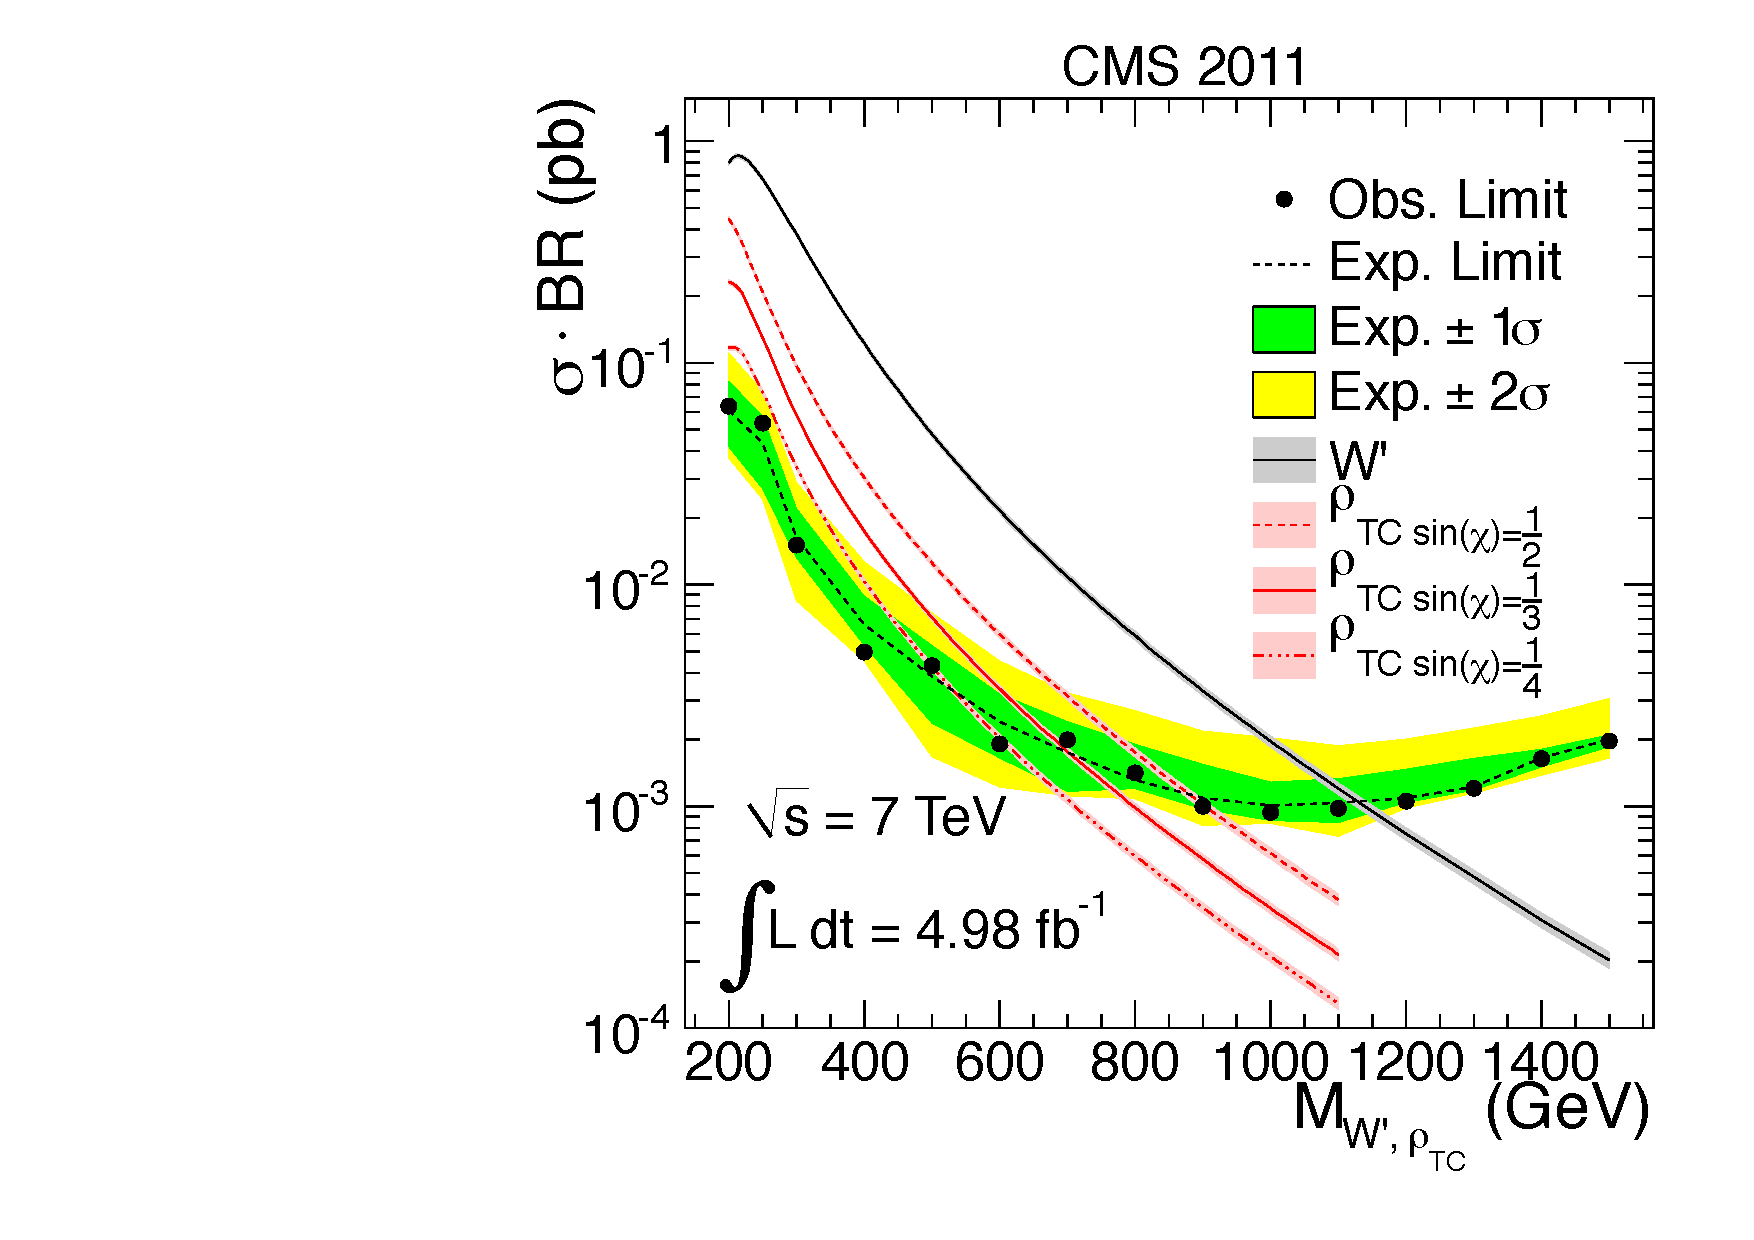
\includegraphics[width=\plotwidth]{figures/limit-vs-mass}
  \caption[Expected and observed upper limits on cross sections as a function of resonance mass]{Expected and observed 95\% C.L.\ upper limits on cross sections as a function of resonance mass for \wprime and \technirho along with the combined statistical and systematic uncertainties depicted with dark green (\SI{1}{$\sigma$}) and light yellow (\SI{2}{$\sigma$}) bands.  The theoretical cross sections (with bands showing the associated PDF uncertainty) include a mass-dependent NNLO $k$-factor.}
  \label{fig:limit-vs-mass}
\end{figure}

It has recently been suggested~\cite{Eichten:2012br} that investigations into Low-Scale Technicolor should evaluate the cross section for $\technirho \to W + Z$ as a function of the model parameter $\sin(\chi)$ since its value has a significant impact on the branching ratios for $\technirho \to W + Z$ and $\technirho \to W + \technipi$, among others.  We take $\sin(\chi) = \frac{1}{3}$ as our nominal value for limit calculations, but additional bands for $\sin(\chi) = \frac{1}{2}$ and $\sin(\chi) = \frac{1}{4}$ are shown in Fig.~\ref{fig:limit-vs-mass}.

\begin{figure}
  \centering
  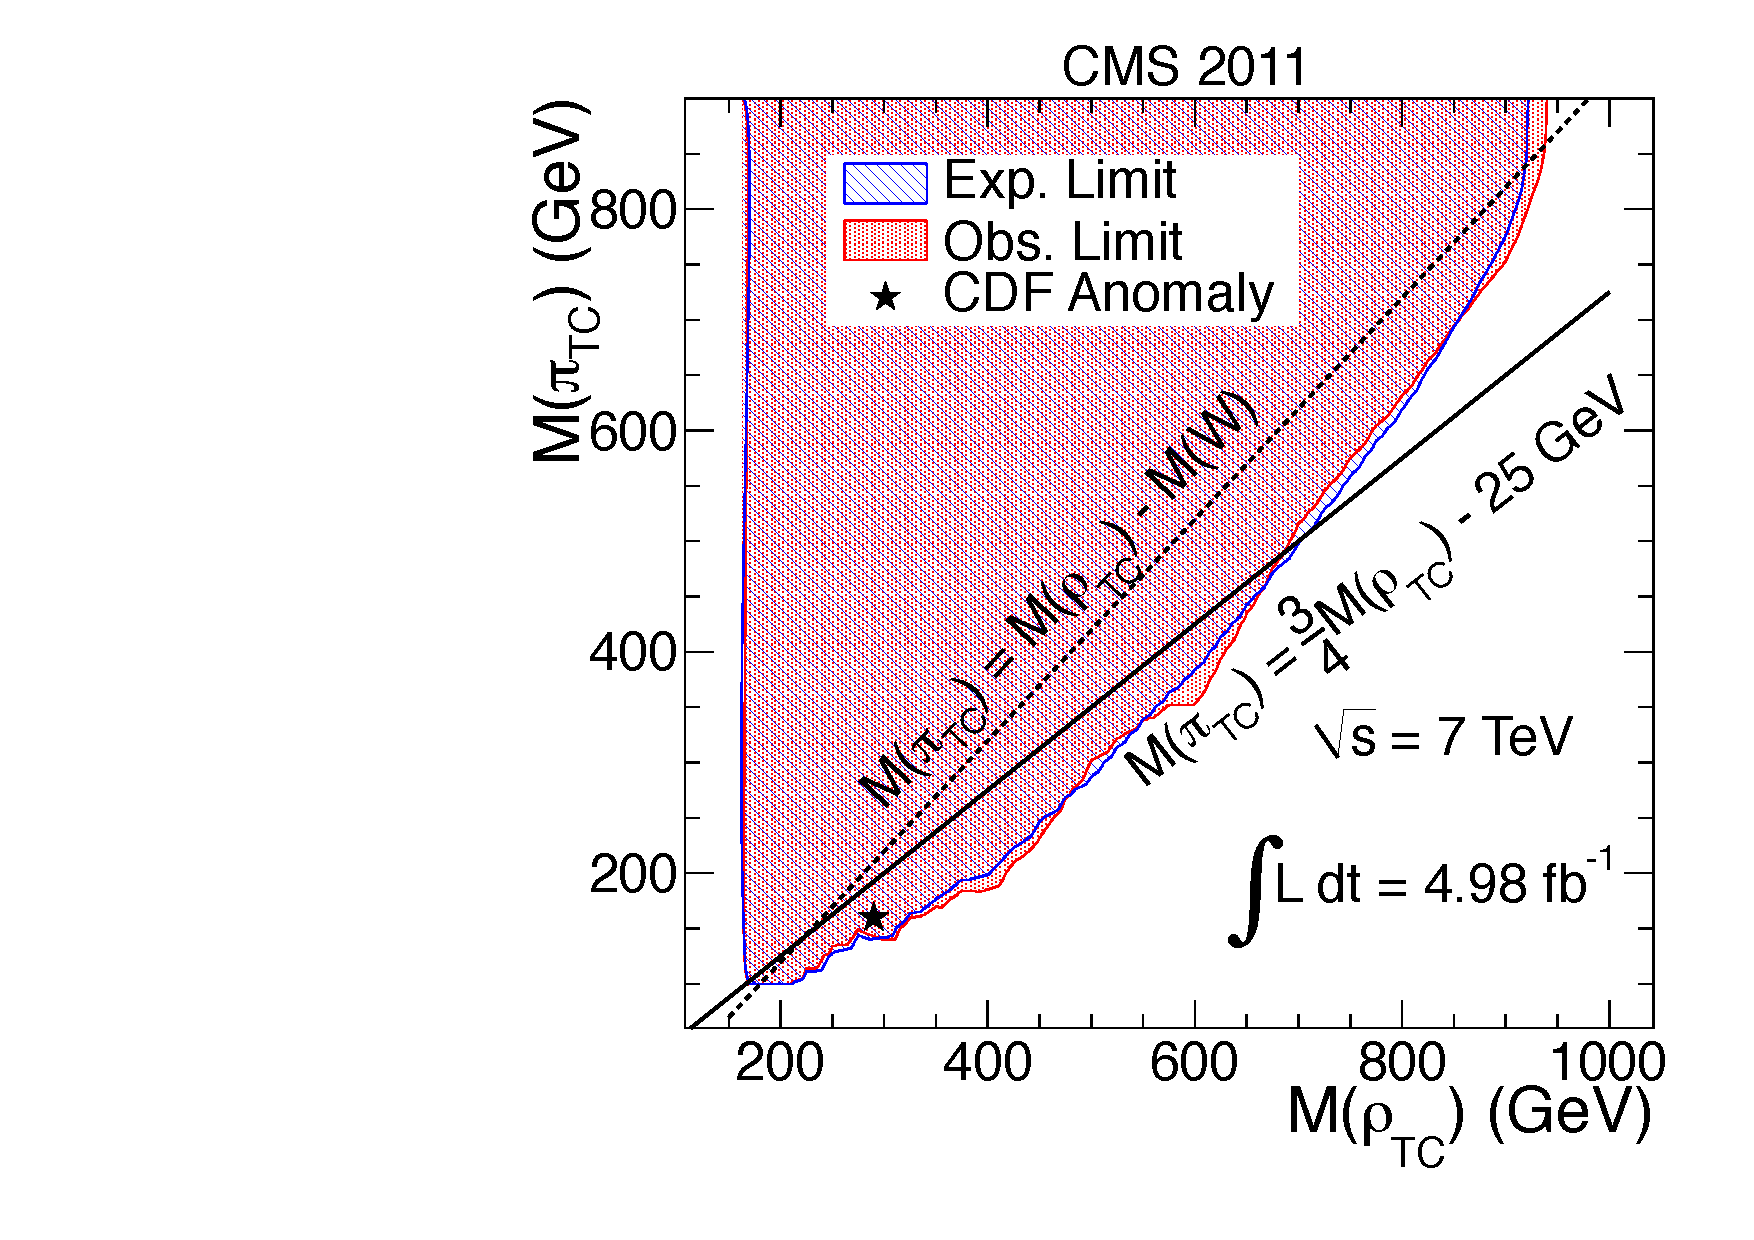
\includegraphics[width=\plotwidth]{figures/tclimit-2d}
  \caption{Exclusion limits for Low-Scale Technicolor as a function of the \technirho and \technipi masses.  The proposed Technicolor interpretation of the CDF anomaly lies inside the excluded region.}
  \label{fig:tclimit-2d}
\end{figure}

One final configuration of interest for Technicolor is motivated by the observation of an excess in the invariant mass spectrum for pairs of jets produced in association with a $W$ boson by the CDF experiment~\cite{Aaltonen:2011mk}.  Many sources have offered interpretations of this ``CDF anomaly'' in terms of new physics models, including a Technicolor configuration with tightly constrained masses for the \technirho (\simass{290}) and \technipi (\simass{160})~\cite{Eichten:2012br}.  For this particular value of $M(\technirho)$, our results place a 95\% \conflevel{} upper bound of \simass{150} for the \technipi mass, barely excluding the Technicolor interpretation.
